\section{Constant Coefficient Equations with Piecewise Continuous Forcing Functions}

\noindent
We'll now consider initial value problems of the form
\begin{equation}\label{eq:8.5.1}
 ay''+by'+cy=f(t), \quad  y(0)=k_0,\quad y'(0)=k_1,
\end{equation}
where $a$, $b$, and $c$ are constants ($a\ne0$) and $f$ is piecewise
continuous on $[0,\infty)$. Problems of this kind occur in situations
where the input to a physical system undergoes instantaneous changes,
as when a switch is turned on or off or the forces acting on the
system change abruptly.

It can be shown (Exercises~\ref{exer:8.5.23} and \ref{exer:8.5.24}) that the
differential equation in \eqref{eq:8.5.1} has no solutions on
an open interval that contains a jump discontinuity of $f$. Therefore we
must define what we mean by a solution of \eqref{eq:8.5.1} on $[0,\infty)$
in the case where $f$ has jump discontinuities. The next theorem
motivates our definition. We omit the proof.

\begin{theorem}\color{blue}\label{thmtype:8.5.1}
Suppose $a,b$, and $c$ are constants $(a\ne0),$ and $f$ is
piecewise  continuous on $[0,\infty).$ with jump discontinuities
at $t_1,$ \dots, $t_n,$ where
$$
0<t_1<\cdots<t_n.
$$
 Let $k_0$ and $k_1$ be arbitrary real numbers. Then there
is a unique function $y$ defined on $[0,\infty)$ with these
properties:
\begin{alist}
\item % (a)
 $y(0)=k_0$ and  $y'(0)=k_1$.
\item % (b)
 $y$ and $y'$  are continuous on $[0,\infty)$.
\item % (c)
$y''$ is defined
on every open subinterval of $[0,\infty)$ that does not contain any of the
points $t_1,$ \dots, $t_n$, and
$$
ay''+by'+cy=f(t)
$$
on every such subinterval.
\item % (d)
$y''$ has limits from the right and left at $t_1,$ \dots$,$ $t_n$.
\end{alist}
\end{theorem}

We define the function $y$  of Theorem~\ref{thmtype:8.5.1}  to be the
solution of the initial value problem \eqref{eq:8.5.1}.

We begin by considering initial value problems of the form
\begin{equation}\label{eq:8.5.2}
ay''+by'+cy=\left\{\begin{array}{cl} f_0(t),&0\le
t<t_1,\\[1\jot]f_1(t),&t\ge t_1,
\end{array}\right.\quad y(0)=k_0,\quad y'(0)=k_1,
\end{equation}
where the forcing function has a single jump discontinuity at $t_1$.

We can solve \eqref{eq:8.5.2} by  the these steps:
\begin{description}
\item{\bf Step 1.} Find the solution $y_0$ of  the initial value problem
$$
ay''+by'+cy=f_0(t), \quad  y(0)=k_0,\quad y'(0)=k_1.
$$
\item{\bf Step 2.} Compute $c_0=y_0(t_1)$ and $c_1=y_0'(t_1)$.
\item{\bf Step 3.} Find the solution $y_1$ of  the initial value problem
$$
ay''+by'+cy=f_1(t), \quad  y(t_1)=c_0,\quad y'(t_1)=c_1.
$$
\item{\bf Step 4.} Obtain the solution $y$ of  \eqref{eq:8.5.2} as
$$
y=\left\{\begin{array}{cl} y_0(t),&0\le t<t_1\\[1\jot]y_1(t),&t\ge t_1.
\end{array}\right.
$$
\end{description}

It is shown  in  Exercise~\ref{exer:8.5.23} that $y'$  exists and is
continuous at $t_1$. The next example illustrates this procedure.

\begin{example}\label{example:8.5.1}\rm
Solve the initial value problem
\begin{equation}\label{eq:8.5.3}
y''+y=f(t),
\quad   y(0)=2,\;  y'(0)=-1,
\end{equation}
where
$$
f(t)=\left\{\begin{array}{rl}
1,&0\le t<\displaystyle{\pi\over2},\\[2\jot]
-1,&t\ge\displaystyle{{\pi\over2}}.
\end{array}\right.
$$
\end{example}

\solution
The  initial value problem in Step 1 is
$$
y''+y=1, \quad   y(0)=2,\quad y'(0)=-1.
$$
We leave it to you to verify that its solution is
$$
y_0=1+\cos t-\sin t.
$$
Doing Step 2 yields
 $y_0(\pi/2)=0$ and $y_0'(\pi/2)=-1$,
so the second initial value problem is
$$
y''+y=-1, \quad  y\left({\pi\over2}\right)=0,\;  y'\left({\pi\over
2}\right)=-1.
$$
We leave it to you to verify that the solution of this problem
is
$$
y_1=-1+\cos t+\sin t.
$$
Hence, the solution of \eqref{eq:8.5.3} is
\begin{equation}\label{eq:8.5.4}
y=\left\{\begin{array}{rl}
1+\cos t-\sin t,&0\le t<\displaystyle{{\pi\over2}},
\\[2\jot]
-1+\cos t+\sin t,&t\ge\displaystyle{{\pi\over2}}
\end{array}\right.
\end{equation}
(Figure:8.5.1).

                    \begin{figure}[tbp]
  \centering\color{blue}
  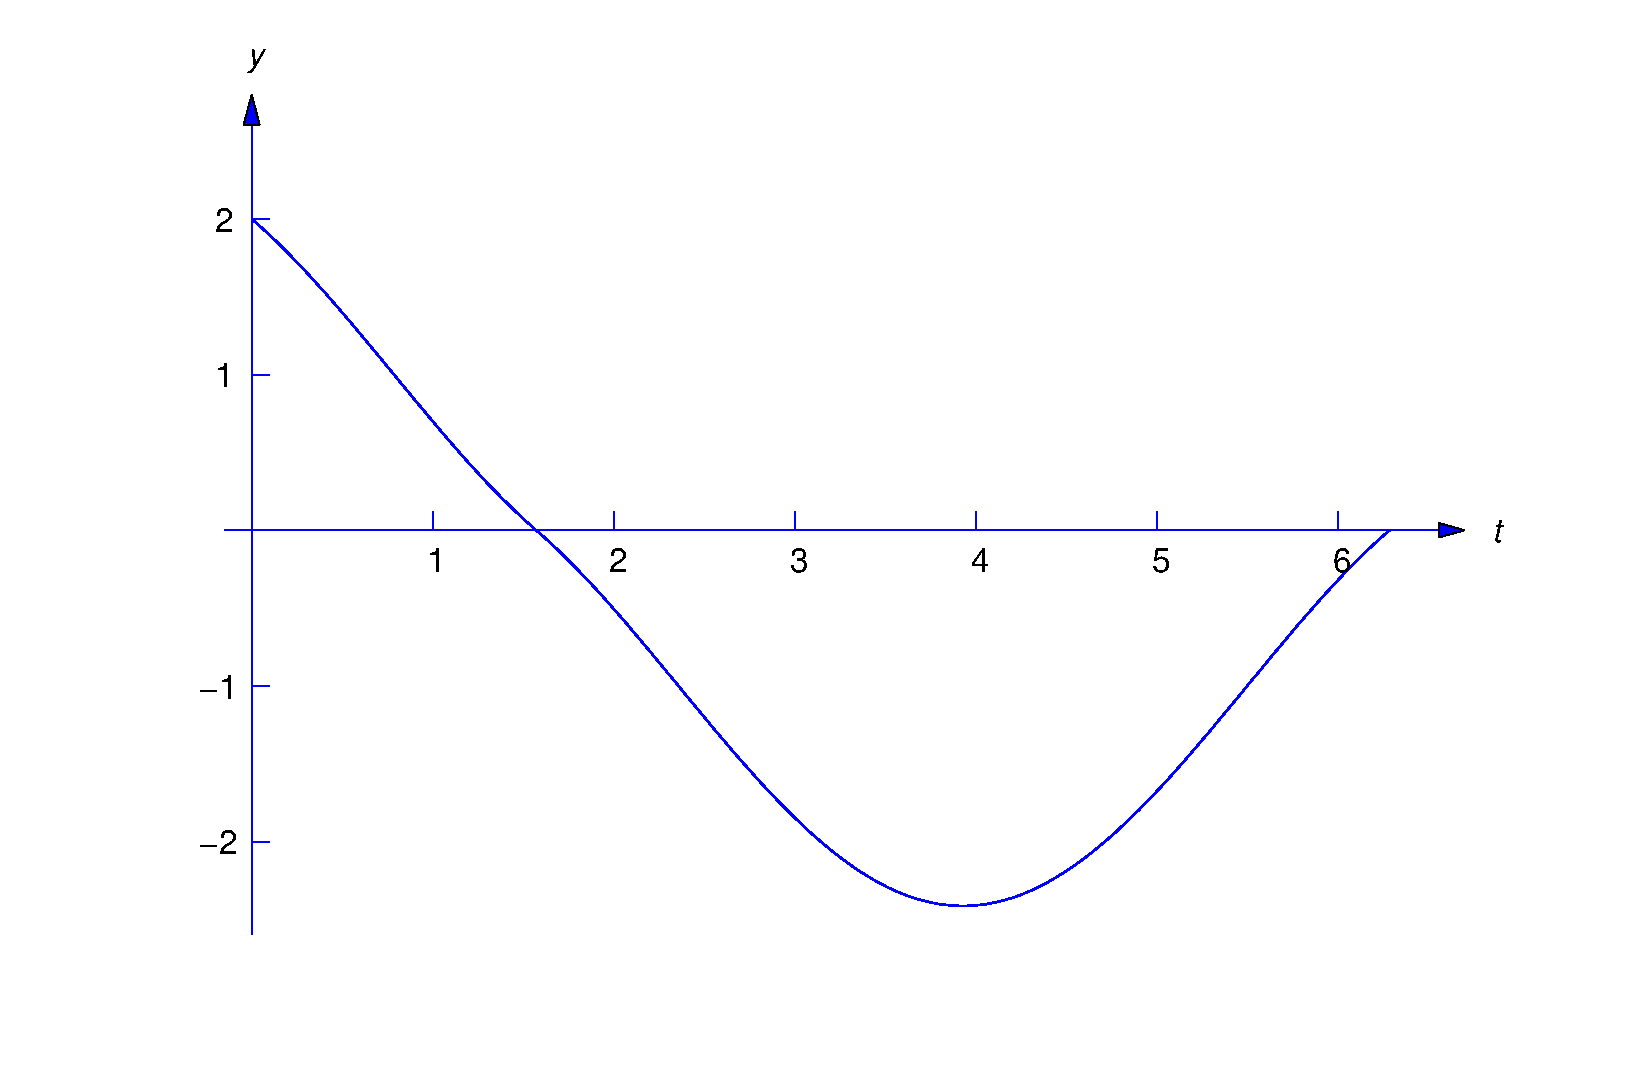
\includegraphics[bb=-78 148 689 643,width=5.67in,height=3.66in,keepaspectratio]{fig080501}
  \caption{ Graph of \eqref{eq:8.5.4}}
  \label{figure:8.5.1}
\end{figure}

If $f_0$ and $f_1$ are defined on $[0,\infty)$, we can rewrite
\eqref{eq:8.5.2} as
$$
ay''+by'+cy=f_0(t)+u(t-t_1)\left(f_1(t)-f_0(t)\right), \quad  y(0)=k_0,\quad y'(0)=k_1,
$$
and apply the method of Laplace transforms. We'll now solve
the problem considered in Example~\ref{example:8.5.1} by this method.

\begin{example}\label{example:8.5.2}\rm
\space Use the Laplace transform to solve the initial value problem
\begin{equation}\label{eq:8.5.5}
y''+y=f(t), \quad   y(0)=2,\;  y'(0)=-1,
\end{equation}
where
$$
f(t)=\left\{\begin{array}{cl}
\phantom{-}1,&0\le t<\dst{{\pi\over2}},\\
-1,&t\ge\dst{{\pi\over2}}.
\end{array}\right.
$$
\end{example}

\solution Here
$$
f(t)=1-2u\left(t-{\pi\over2}\right),
$$
so Theorem~\ref{thmtype:8.4.1} (with $g(t)=1$) implies that
$$
{\cal L}(f)={1-2e^{-{\pi s/2}}\over s}.
$$
Therefore, transforming  \eqref{eq:8.5.5} yields
$$
(s^2+1)Y(s)={1-2e^{-{\pi s/ 2}}\over s}-1+2s,
$$
 so
\begin{equation}\label{eq:8.5.6}
Y(s)=(1-2e^{-{\pi s/ 2}}) G(s)+{2s-1\over s^2+1},
\end{equation}
with
$$
G(s)={1\over s(s^2+1)}.
$$
The  form for the partial fraction expansion of $G$ is
\begin{equation}\label{eq:8.5.7}
{1\over s(s^2+1)}={A\over s}+{Bs+C\over s^2+1}.
\end{equation}
Multiplying through by $s(s^2+1)$ yields
$$
A(s^2+1)+(Bs+C)s=1,
$$
or
$$
(A+B)s^2+Cs+A=1.
$$
Equating coefficients of like powers of $s$ on the two sides of this
equation shows that $A=1$, $B=-A=-1$ and $C=0$. Hence, from
\eqref{eq:8.5.7},
$$
G(s)={1\over s}-{s\over s^2+1}.
$$
Therefore
$$
g(t)=1-\cos t.
$$
From this,  \eqref{eq:8.5.6}, and
Theorem~\ref{thmtype:8.4.2},
$$
y=1-\cos t-2u\left(t-{\pi\over2}\right)\left(1-\cos\left(t-{\pi
\over2}\right)\right)+2\cos t-\sin t.
$$
Simplifying this (recalling that $\cos (t-\pi/2)=\sin t)$ yields
$$
y=1+\cos t-\sin t-2u\left(t-{\pi\over2}\right)(1-\sin t),
$$
or
$$
y=\left\{\begin{array}{cl}
\phantom{-} 1+\cos t-\sin t,&0\le t<\dst{{\pi\over2}},\\
-1+\cos t+\sin t,&t\ge\dst{{\pi\over2}},
\end{array}\right.
$$
which is the result obtained in Example~\ref{example:8.5.1}.

\medskip
\color{blue}
\remark{It isn't obvious that using the Laplace transform to solve
\eqref{eq:8.5.2} as we did in Example~\ref{example:8.5.2} yields a function
$y$ with the properties stated in Theorem~\ref{thmtype:8.5.1}; that is,
such that $y$ and $y'$ are continuous on $[0,\infty)$ and $y''$ has
limits from the right and left at $t_1$. However, this is
true if  $f_0$ and $f_1$ are continuous and of exponential order on
$[0,\infty)$. A proof  is sketched in
Exercises~8.6.~\hspace*{-3pt}\ref{exer:8.6.11}--8.6.\hspace*{-3pt}\ref{exer:8.6.13}.}
\color{black}

\begin{example}\label{example:8.5.3}\rm
\space Solve the initial value problem
\begin{equation}\label{eq:8.5.8}
y''-y=f(t), \quad   y(0)=-1,\;  y'(0)=2,
\end{equation}
where
$$
f(t)=\left\{\begin{array}{cl}
t,&0\le t<1,\\
1,&t\ge 1.
\end{array}\right.
$$
\end{example}

\solution  Here
$$
f(t)=t-u(t-1)(t-1),
$$
so
\begin{eqnarray*}
{\cal L}(f)&=&{\cal L}(t)-{\cal L}\left(u(t-1)(t-1)\right)\\[1\jot]
&=&{\cal L}(t)-e^{-s}{\cal L}(t)\mbox{ (from
Theorem~\ref{thmtype:8.4.1})}\\[1\jot]
&=&{1\over s^2}-{e^{-s}\over s^2}.
\end{eqnarray*}
Since transforming  \eqref{eq:8.5.8} yields
$$
(s^2-1) Y(s)={\cal L}(f)+2-s,
$$
we see that
\begin{equation}\label{eq:8.5.9}
Y(s)=(1-e^{-s})H(s)+{2-s\over s^2-1},
\end{equation}
where
$$
H(s)={1\over s^2(s^2-1)}={1\over s^2-1}-{1\over s^2};
$$
 therefore
\begin{equation}\label{eq:8.5.10}
h(t)=\sinh t-t.
\end{equation}
Since
$$
{\cal L}^{-1}\left({2-s\over s^2-1}\right)=2\sinh t-\cosh t,
$$
we conclude from  \eqref{eq:8.5.9},  \eqref{eq:8.5.10}, and
Theorem~\ref{thmtype:8.4.1} that
$$
y=\sinh t-t-u(t-1)\left(\sinh (t-1)-t+1\right)+2\sinh t-
\cosh t,
$$
or
\begin{equation}\label{eq:8.5.11}
y=3\sinh t-\cosh t-t-u(t-1)\left(\sinh (t-1)-t+1\right)
\end{equation}
We leave it to you to verify that $y$  and $y'$ are continuous and
$y''$ has limits from the right and left at
$t_1=1$.

\begin{example}\label{example:8.5.4}\rm
 Solve the initial value problem
\begin{equation}\label{eq:8.5.12}
y''+y=f(t), \quad   y(0)=0,\;  y'(0)=0,
\end{equation}
where
$$
f(t)=\left\{\begin{array}{cl}
 0,&0\le t<\dst{{\pi\over4}},\\[2\jot]
\cos2t,&\dst{{\pi\over4}}\le t<\pi,\\[2\jot]
 0,&t\ge\pi.
\end{array}\right.
$$
\end{example}

\solution  Here
$$
f(t)=u(t-\pi/4)\cos2t-u(t-\pi)\cos2t,
$$
so
\begin{eqnarray*}
{\cal L}(f)&=&{\cal L}\left(u(t-\pi/4)\cos2t\right)-{\cal L}\left(
u(t-\pi)\cos2t\right)\\[1\jot]
&=&e^{-{\pi s/4}}{\cal L}\left(\cos2(t+\pi/4)\right)-e^{-\pi s}
{\cal L}\left(\cos2(t+\pi)\right)\\[1\jot]
&=&-e^{-{\pi s/4}}{\cal L}(\sin2t)-e^{-\pi s}
{\cal L}(\cos2t)\\[1\jot]
&=&-{2e^{-{\pi s/ 4}}\over s^2+4}-{se^{-\pi s}\over s^2+4}.
\end{eqnarray*}
Since transforming  \eqref{eq:8.5.12} yields
$$
(s^2+1)Y(s)={\cal L}(f),
$$
we see that
\begin{equation}\label{eq:8.5.13}
Y(s)=e^{-{\pi s/ 4}} H_1(s)+e^{-\pi s} H_2(s),
\end{equation}
where
\begin{equation}\label{eq:8.5.14}
H_1(s)=-{2\over (s^2+1)(s^2+4)}\quad\mbox{ and }\quad H_2(s)=-{s
\over
(s^2+1)(s^2+4)}.
\end{equation}
To simplify the required partial fraction expansions, we first write
$$
{1\over (x+1)(x+4)}={1\over3}\left[{1\over x+1}-{1\over
x+4}\right].
$$
Setting $x=s^2$ and substituting the result in  \eqref{eq:8.5.14} yields
$$
H_1(s)=-{2\over3}\left[{1\over s^2+1}-{1\over s^2+4}\right]
\quad\mbox{ and }\quad
H_2(s)=-{1\over3}\left[{s\over s^2+1}-{s\over s^2+4}\right].
$$
The inverse transforms are
$$
h_1(t)=-{2\over3}\sin t+{1\over3}\sin2t
\quad\mbox{ and }\;
h_2(t)=-{1\over3}\cos t+{1\over3}\cos2t.
$$
From  \eqref{eq:8.5.13} and Theorem~8.4.2,
\begin{equation}\label{eq:8.5.15}
y=u\left(t-{\pi\over4}\right) h_1\left(t-{\pi\over4}\right)+
u(t-\pi) h_2(t-\pi).
\end{equation}
Since
\begin{eqnarray*}
h_1\left(t-{\pi\over4}\right)&=&-{2\over3}\sin\left(t-{\pi\over
4}\right)+{1\over3}\sin2\left(t-{\pi\over4}\right)\\
&=&-{\sqrt{2}\over3} (\sin t-\cos t)-{1\over3}\cos2t
\end{eqnarray*}
and
\begin{eqnarray*}
h_2(t-\pi)&=&-{1\over3}\cos (t-\pi)+{1\over3}\cos2(t-\pi)\\
&=&{1\over3}\cos t+{1\over3}\cos2t,
\end{eqnarray*}
 \eqref{eq:8.5.15} can be rewritten as
$$
y=-{1\over3}u\left(t-{\pi\over4}\right)\left(\sqrt{2}(\sin
t-\cos t)+\cos2t\right)
+ {1\over3} u(t-\pi) (\cos t+\cos2t)
$$
or
\begin{equation}\label{eq:8.5.16}
y=\left\{\begin{array}{cl}
0,&0\le t<\dst{{\pi\over4}},\\[2\jot]
-\dst{{\sqrt{2}\over3}}(\sin t-\cos t)-\dst{{1\over
3}}\cos2t,&\dst{\pi\over4}\le t<\pi,\\[2\jot]
-\dst{ {\sqrt{2}\over3}}\sin t+
\dst{{1+\sqrt{2}\over3}}\cos t ,&t\ge\pi.
\end{array}\right.
\end{equation}
We leave it to you to verify that $y$ and $y'$ are continuous and
$y''$ has limits from the right and left at $t_1=\pi/4$ and $t_2=\pi$
(Figure~\ref{figure:8.5.2}).

\begin{figure}[tbp]
  \centering\color{blue}
  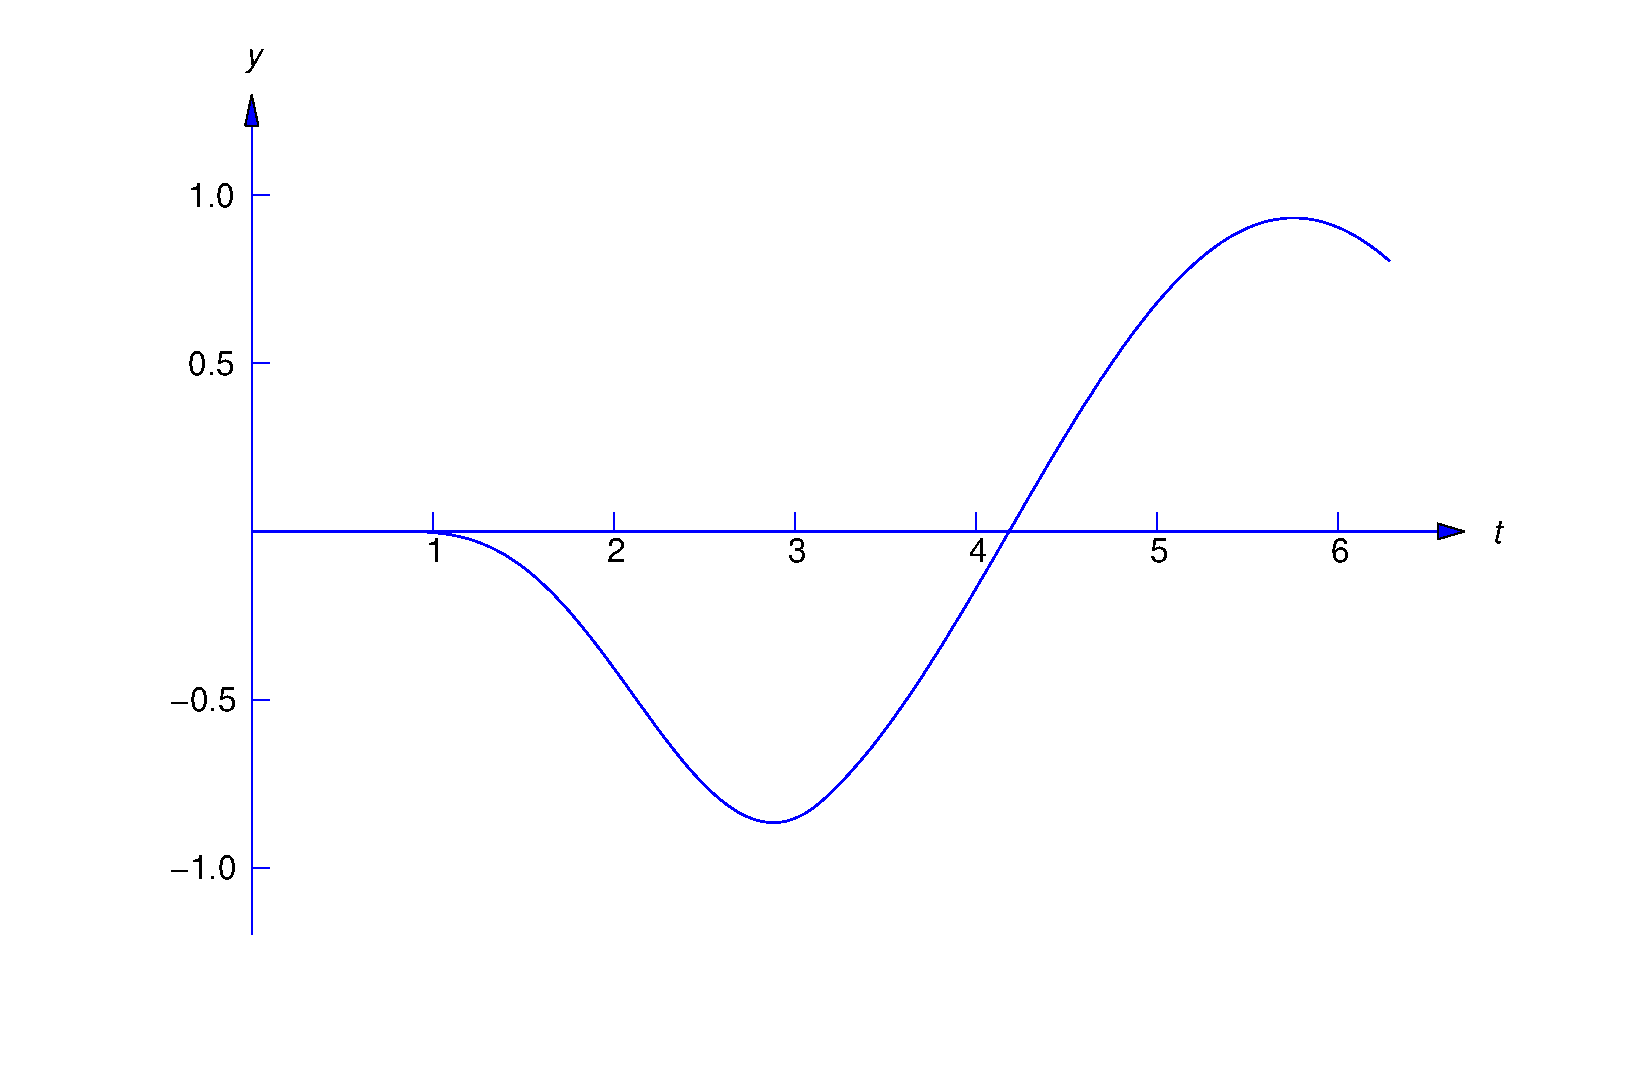
\includegraphics[bb=-78 148 689 643,width=5.67in,height=3.66in,keepaspectratio]{fig080502}
  \caption{ Graph of \eqref{eq:8.5.16}}
  \label{figure:8.5.2}
\end{figure}

\exercises
\noindent In Exercises~\ref{exer:8.5.1}--\ref{exer:8.5.20} use the Laplace
transform to solve the initial value problem.
Where indicated by\\ \CGex, graph the solution.

\begin{exerciselist}

\item\label{exer:8.5.1} $\dst{y''+y=\left\{\begin{array}{cl} 3,& 0\le
t<\pi,\\[2\jot] 0,&t\ge\pi,\end{array}\right.\qquad y(0)=0, \quad  y'(0)=0}$

\item\label{exer:8.5.2} $\dst{y''+y=\left\{\begin{array}{cl} 3,&0\le
t<4,\\; 2t-5,&t > 4,\end{array}\right.\qquad y(0)=1,\quad y'(0)=0}$

\item\label{exer:8.5.3} $\dst{y''-2y'= \left\{\begin{array}{cl} 4,&0\le
t<1,\\[2\jot] 6,&t\ge 1,\end{array}\right.\qquad y(0)=-6,\quad y'(0)=1 }$

\item\label{exer:8.5.4} $\dst{y''-y=\left\{\begin{array}{cl} e^{2t},&0\le
t< 2,\\[2\jot] 1,&t\ge 2,\end{array}\right.\qquad y(0)=3,\quad y'(0)=-1
}$

\item\label{exer:8.5.5} $\dst{y''-3y'+2y= \left\{\begin{array}{rl} 0,&0\le
t<1,\\[2\jot] 1,&1\le t<2,\\[2\jot]-1,&t\ge 2,
\end{array}\right.\qquad y(0)=-3,\quad y'(0)=1}$

\item\label{exer:8.5.6} \CGex $\dst{y''+4y= \left\{\begin{array}{cl}|\sin
t|,&0\le t<2\pi,\\[2\jot] 0,&t\ge 2\pi,\end{array}\right.\qquad
y(0)=-3,\quad y'(0)=1}$

\item\label{exer:8.5.7} $\dst{y''-5y'+4y= \left\{\begin{array}{rl} 1,&0\le
t<1\\[2\jot] -1,&1\le t<2,\\[2\jot] 0,&t\ge 2,\end{array}\right.\qquad
y(0)=3,\quad y'(0)=-5}$

\item\label{exer:8.5.8} $\dst{y''+9y= \left\{\begin{array}{cl} \cos
t,&0\le t<\dst{{3\pi\over2}},\\[2\jot] \sin
t,&t\ge\dst{{3\pi\over2}},\end{array}\right.\qquad y(0)=0,\;  y'(0)=0}$

\item\label{exer:8.5.9} \CGex $\dst{y''+4y= \left\{\begin{array}{cl} t,&0\le
t<\dst{\pi \over2},\\[2\jot]\pi,&t\ge\dst{ {\pi\over2}},
\end{array}\right.\quad y(0)=0,\quad y'(0)=0}$

\item\label{exer:8.5.10}
$\dst{y''+y=\left\{\begin{array}{cl}\phantom{-}t,&0\le t<\pi,
\\[2\jot]-t,&t\ge\pi ,\end{array}\right.\;  y(0)=0,\;  y'(0)=0}$

\item\label{exer:8.5.11} $\dst{y''-3y'+2y=\left\{\begin{array}{cl} 0,&0\le
t<2,\\2t-4,&t\ge 2,\end{array}\right. ,\quad y(0)=0,\quad y'(0)=0}$

\item\label{exer:8.5.12} $\dst{y''+y=\left\{\begin{array}{cl} t,&0\le
t<2\pi,\\-2t,&t\ge 2\pi,\end{array}\right.\quad y(0)=1,\quad y'(0)=2}$

\item\label{exer:8.5.13} \CGex
$\dst{y''+3y'+2y=\left\{\begin{array}{cl}\phantom{-}1,&0\le
t<2,\\-1,&t\ge 2,\end{array}\right.\;  y(0)=0,\;  y'(0)=0}$

\item\label{exer:8.5.14} $\dst{y''-4y'+3y=\left\{\begin{array}{cl}-1,&0\le
t<1,\\\phantom{-}1,&t\ge 1,\end{array}\right.\;  y(0)=0,\;  y'(0)=0}$

\item\label{exer:8.5.15} $\dst{y''+2y'+y=\left\{\begin{array}{cl}
e^t,&0\le t<1,\\e^t-1,&t\ge 1,\end{array}\right.\;  y(0)=3,\;
y'(0)=-1}$

\item\label{exer:8.5.16}
 $\dst{y''+2y'+y=\left\{\begin{array}{cl}
4e^t,&0\le t<1,\\0,&t\ge 1,\end{array}\right.\;  y(0)=0,\;
y'(0)=0}$

\item\label{exer:8.5.17} $\dst{y''+3y'+2y=\left\{\begin{array}{cl}
e^{-t},&0\le t<1,\\0,&t\ge 1,\end{array}\right.\;  y(0)=1,\;  y'(0)=-1}$

\item\label{exer:8.5.18} $\dst{y''-4y'+4y=\left\{\begin{array}{rl}
e^{2t},&0\le t<2,\\-e^{2t},&t\ge 2,\end{array}\right.\;  y(0)=0,\;
y'(0)=-1}$

\item\label{exer:8.5.19} \CGex $\dst{y''=\left\{\begin{array}{cl}t^2,&0\le
t<1,\\-t,&1\le t<2,\\t+1,&t\ge 2,\end{array}\right.\;  y(0)=1,\;
y'(0)=0}$

\item\label{exer:8.5.20} $\dst{y''+2y'+2y=\left\{\begin{array}{rl}1,&0\le
t<2\pi,\\t,&2\pi\le t<3\pi,\\-1,&t\ge 3\pi,\end{array}\right.\;
y(0)=2,\quad y'(0)=-1}$

\item\label{exer:8.5.21} Solve the initial value problem $$ y''=f(t), \quad
y(0)=0,\quad  y'(0)=0, $$ where $$ f(t)=m+1,\quad m\le t<m+1,\quad
m=0,1,2,\dots. $$

\item\label{exer:8.5.22} Solve the given initial value problem and find a
formula that does not involve step functions and represents $y$ on
each interval of continuity of $f$.
\begin{alist}
\item % (a)
$y''+y=f(t), \quad  y(0)=0,\quad  y'(0)=0$;

$f(t)=m+1,\quad  m\pi\le t<(m+1)\pi,\quad m=0,1,2,\dots$.

\item % (b)
$y''+y=f(t), \quad  y(0)=0,\quad y'(0)=0$;

$f(t)=(m+1)t, \quad   2m\pi\le t<2(m+1)\pi,\quad m=0,1,2,\dots$
\hint{You'll need the formula}
$$
1+2+\cdots+m={m(m+1)\over2}.
$$

\item % (c)
$y''+y=f(t), \quad  y(0)=0,\quad  y'(0)=0$;

$f(t)=(-1)^m,\quad  m\pi\le t<(m+1)\pi,\quad m=0,1,2,\dots.$

\item % (d)
$y''-y=f(t), \quad  y(0)=0,\quad  y'(0)=0$;

$f(t)=m+1,\quad  m\le t<(m+1),\quad m=0,1,2,\dots.$

\hint{You will need the formula
$$
1+r+\cdots+r^m={1-r^{m+1}\over1-r}\; (r\ne1).
$$}

\item % (d)
$y''+2y'+2y=f(t), \quad  y(0)=0,\quad  y'(0)=0$;

$f(t)=(m+1)(\sin t+2\cos t),\quad  2m\pi\le t<2(m+1)\pi,\quad
m=0,1,2,\dots.$

(See the hint in \part{d}.)

\item % (f)
$y''-3y'+2y=f(t), \quad  y(0)=0,\quad y'(0)=0$;

$f(t)=m+1,\quad  m\le t<m+1,\quad m=0,1,2,\dots.$

 (See the hints in \part{b} and \part{d}.)
\end{alist}

\item\label{exer:8.5.23}
\begin{alist}
\item % (a)
Let $g$ be  continuous on  $(\alpha,\beta)$
 and differentiable on the  $(\alpha,t_0)$
and $(t_0,\beta)$. Suppose $A=\lim_{t\to t_0-}g'(t)$
and $B=\lim_{t\to t_0+}g'(t)$ both exist. Use the mean value theorem
to show that
$$
\lim_{t\to t_0-}{g(t)-g(t_0)\over t-t_0}=A\quad\mbox{ and }\quad
\lim_{t\to t_0+}{g(t)-g(t_0)\over t-t_0}=B.
$$
\item % (b)
Conclude from \part{a} that $g'(t_0)$ exists and $g'$ is continuous at
$t_0$ if $A=B$.

\item % (c)
Conclude from \part{a}
 that if $g$  is differentiable on $(\alpha,\beta)$ then
$g'$ can't have a jump discontinuity on $(\alpha,\beta)$.
\end{alist}

\item\label{exer:8.5.24}
\begin{alist}
\item % (a)
Let $a$, $b$, and $c$ be constants, with $a\ne0$. Let $f$ be piecewise
continuous on an interval $(\alpha,\beta)$, with a single jump
discontinuity at a point $t_0$ in $(\alpha,\beta)$. Suppose $y$
and $y'$ are continuous on $(\alpha,\beta)$ and $y''$ on
$(\alpha,t_0)$ and $(t_0,\beta)$. Suppose  also that
$$
ay''+by'+cy=f(t)
\eqno{\rm (A)}
$$
on $(\alpha,t_0)$ and $(t_0,\beta)$.
Show that
$$
y''(t_0+)-y''(t_0-)={f(t_0+)-f(t_0-)\over a}\ne0.
$$
\item % (b)
Use \part{a}  and Exercise~\ref{exer:8.5.23}\part{c} to show that
(A)
does not  have  solutions on any interval $(\alpha,\beta)$ that contains
a jump discontinuity of $f$.
\end{alist}

\item\label{exer:8.5.25}
Suppose $P_0,P_1$, and $P_2$ are continuous and $P_0$
has no zeros on an open interval $(a,b)$, and  that $F$
has a jump discontinuity at a point $t_0$ in $(a,b)$.
Show that the differential equation
$$
P_0(t)y''+P_1(t)y'+P_2(t)y=F(t)
$$
has no solutions on $(a,b)$.\hint{Generalize the result of
Exercise~$\ref{exer:8.5.24}$ and use Exercise~$\ref{exer:8.5.23}\part{c}$.}

\item\label{exer:8.5.26}
Let $0=t_0<t_1<\cdots <t_n$. Suppose $f_m$ is continuous
on $[t_m,\infty)$ for $m=1,\dots,n$.
 Let
$$
f(t)=
\left\{\begin{array}{cl}
f_m(t),&t_m\le t< t_{m+1},\quad m=1,\dots,n-1,\\
f_n(t),&t\ge t_n.
\end{array}\right.
$$
Show that the
solution of
$$
ay''+by'+cy=f(t), \quad  y(0)=k_0,\quad y'(0)=k_1,
$$
as defined following  Theorem~8.5.1, is given by
$$
y=\left\{\begin{array}{cl}
 z_0(t),&0\le t<t_1,\\[1\jot]
z_0(t)+ z_1(t),&t_1\le t<t_2,\\
&\vdots\\
z_0+\cdots+z_{n-1}(t),&t_{n-1}\le t<t_n,\\[1\jot]
z_0+\cdots+ z_n(t),&t\ge t_n,
\end{array}\right.
$$
where $z_0$ is the solution of
$$
az''+bz'+cz=f_0(t), \quad  z(0)=k_0,\quad  z'(0)=k_1
$$
and $z_m$ is the solution of
$$
az''+bz'+cz=f_m(t)-f_{m-1}(t), \quad  z(t_m)=0,\quad z'(t_m)=0
$$
for $m=1,\dots,n$.
\end{exerciselist}
